\chapter{Arquitetura da aplicação Zulip}

A arquitetura da aplicação \textbf{zulip} contém vários \textbf{componentes}, sendo que, se consegue dividir os mesmos em diferentes subsistemas. No entanto, é perceptível pela figura \ref{img:arquitetura-zulip}, que existe uma separação entre o componente \textbf{Client} com os restantes, pois são subsistemas distintos.
\newline

\begin{figure}[H]
	\centering
	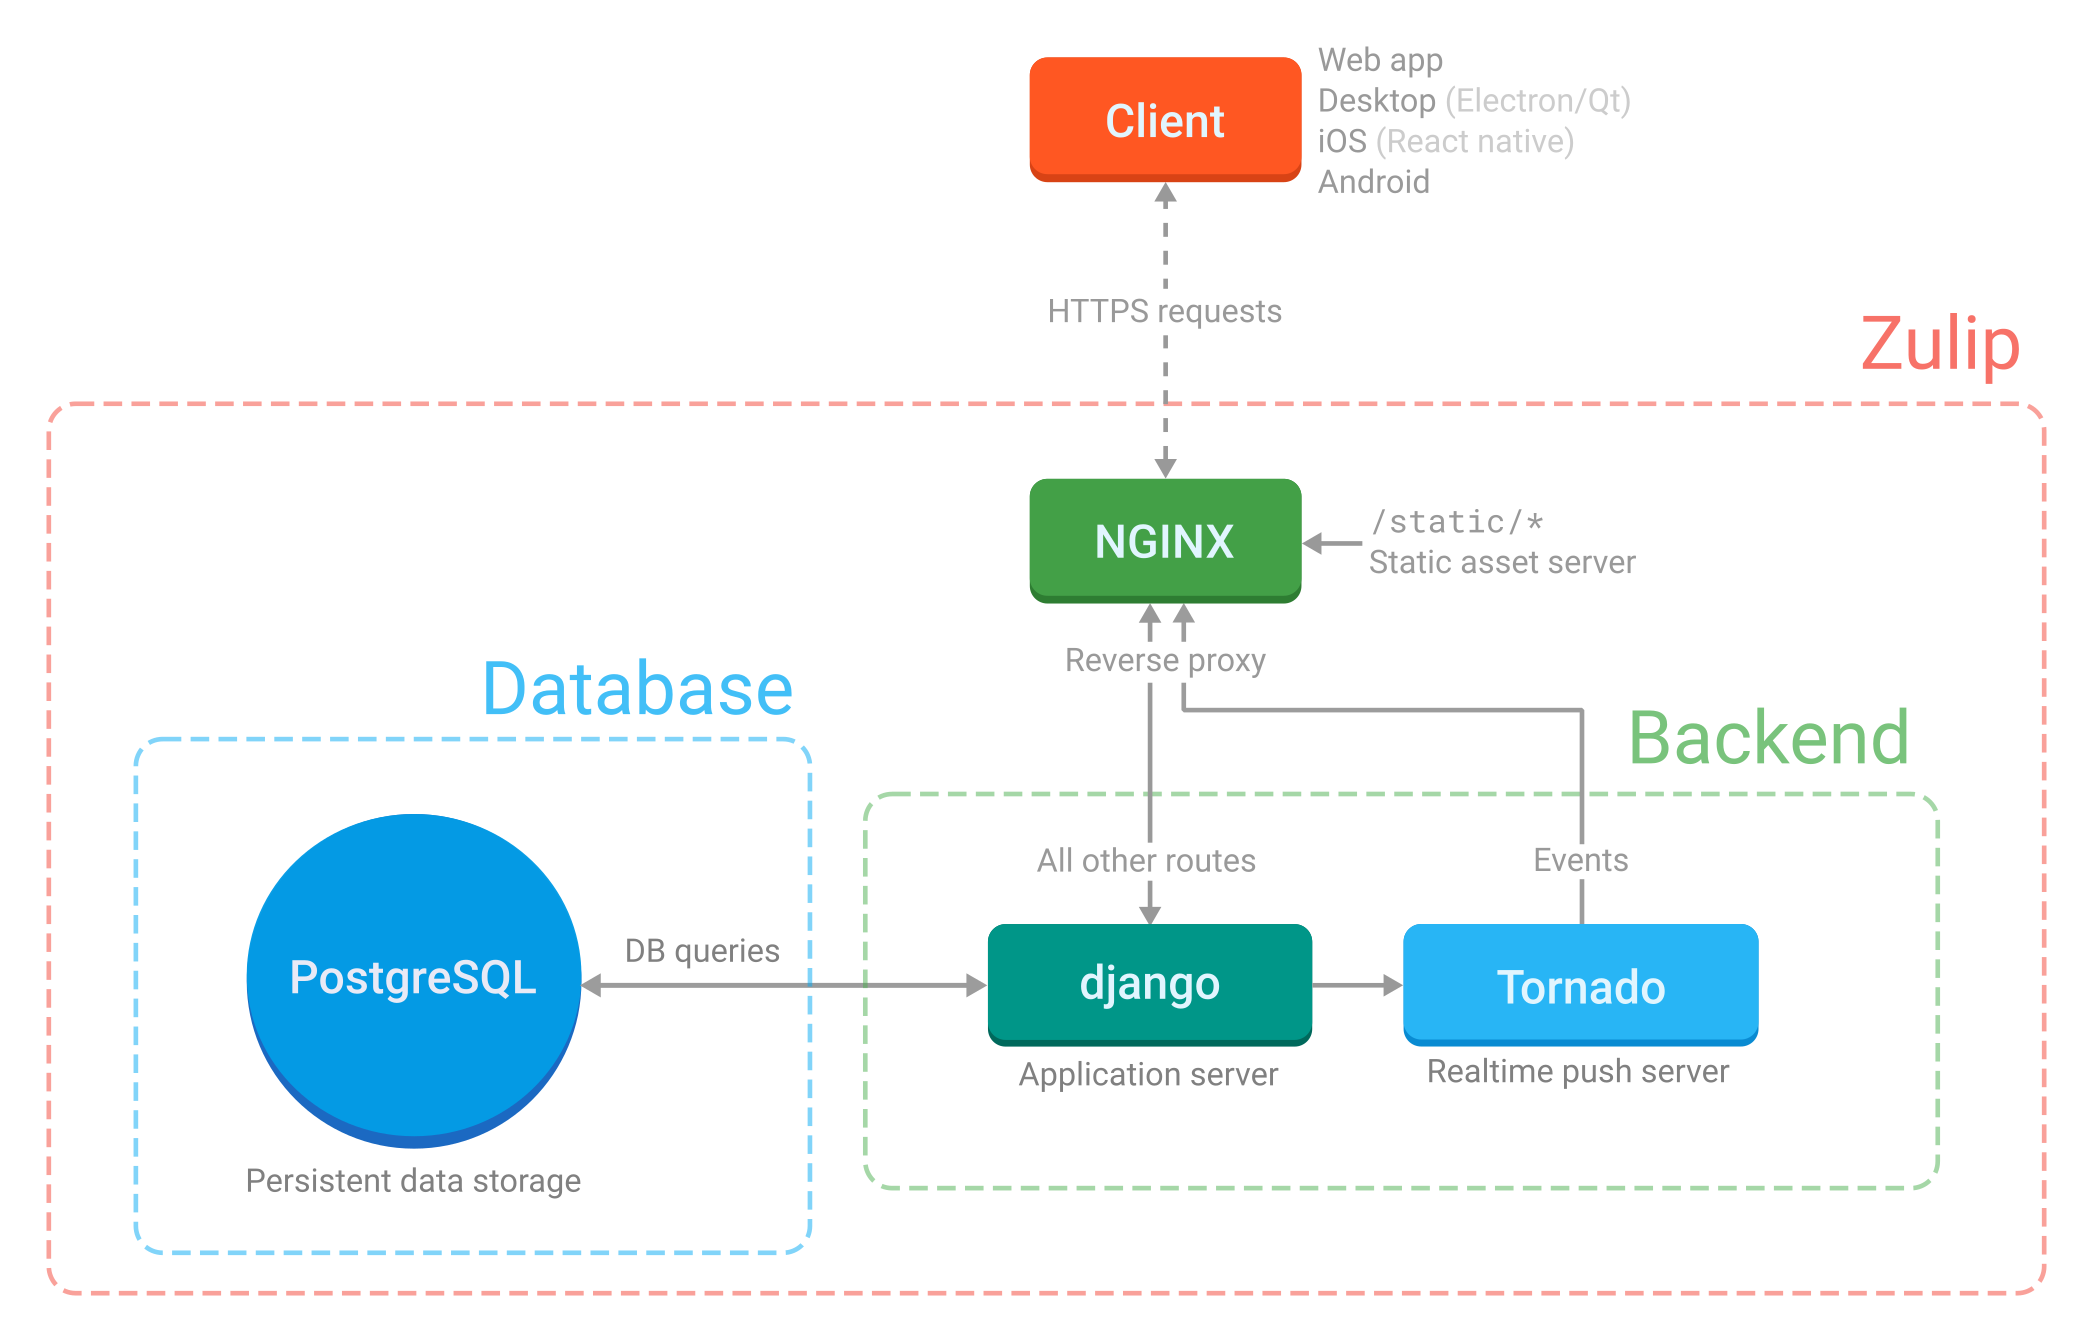
\includegraphics[scale=0.28]{images/architecture.png}
	\caption{\href{https://zulip.readthedocs.io/en/latest/overview/architecture-overview.html}{Arquitetura da aplicação Zulip.}}
	\label{img:arquitetura-zulip}
\end{figure}

O \textbf{Client} é responsável pela apresentação (\emph{view}) da aplicação, enquanto que o restante subsistema é de uma forma geral, responsável pela lógica e tratamento de dados da mesma, sendo este mais complexo e composto por subsistemas interiores (\textbf{Database} \& \textbf{Backend}).
\newline

A divisão também deve-se ao facto do componente \textbf{Client} estar na máquina do utilizador, enquanto que os restantes estarão em máquinas administradas pela empresa de desenvolvimento.
\newline

O componente \textbf{NGINX} consiste num servidor \emph{HTTP} intermediário (\emph{middleware}) entre o componente \textbf{Client} com \emph{HTTP requests} e o \textbf{Backend}. Na verdade, o \textbf{NGINX} permite uma independência entre os subsistemas, ou seja, o \textbf{Client}, pode ser definido para diferentes plataformas, nomeadamente: web, desktop, iOS e android.
\newline

Em relação à base de dados da aplicação, tem-se o componente \textbf{PostgreSQL}, um sistema de gerenciamento de dados persistente que apenas comunica com o servidor da aplicação \textbf{django}.
\newline

Em termos do sistema de \textbf{backend} da aplicação, este é composto por duas componentes, sendo elas \textbf{django} e \textbf{Tornado}, este primeiro \textbf{django} é de extrema importância tendo em conta que é a base da construção da aplicação \textbf{zulip}, e consiste num framework de web do lado do servidor de código aberto, desenvolvido em Python, fornecendo assim todo o framework necessário para ser mais tarde apresentado do lado do cliente, quanto ao \textbf{Tornado} é um servidor de web assíncrono e sem bloqueio de I/o que permite manter ativas milhares de ligações em tempo real, no caso do \textbf{zulip} é respónsavel pela entrega de mensagens e não muito mais.\\ 

Outros componentes secundários igualmente importantes no funcionamento do \textbf{zulip} são \textbf{Supervisor} que é um sistema cliente/servidor que permite monitorizar e controlar os processos em sistemas \textbf{unix}, no caso do \textbf{zulip} é utilizado para iniciar os processos do servidor, reinicializar-los em caso de falha e fazer \emph{logging}, outro é \textbf{memcached} é um sistema distribuído de cache em memória, é usado para guardar em chache modelos de dados e invalidar-los caso sejam alterados.\\

Um outro componente secundário é a base de dados em memória \textbf{Redis} que armazena chaves com durabilidade opcional, é usado para guardar dados com tempo de vida bastante baixo.\\ O \textbf{RabbitMQ} é um software de mensagens com código aberto, que é usado para tratar de filas que requerem uma entrega fiável mas não são passíveis de fazer no sistema principal, é também usado para comunicações entre \textbf{django} e \textbf{Tornado}.\\ Por último, o componente \textbf{Thumbor} é um serviço de miniaturas de fotos open-source que tem como função administrar as fotos do sistemas ora via \textbf{upload} ora via \textbf{url}.\newline

Importante realçar que a arquitetura que será elaborada no deployment da aplicação, varia consoante o número de replicas de cada componente. No entanto isto será abordado com mais detalhe nos capítulos seguintes.